\documentclass[]{article}
\usepackage{lmodern}
\usepackage{amssymb,amsmath}
\usepackage{ifxetex,ifluatex}
\usepackage{fixltx2e} % provides \textsubscript
\ifnum 0\ifxetex 1\fi\ifluatex 1\fi=0 % if pdftex
  \usepackage[T1]{fontenc}
  \usepackage[utf8]{inputenc}
\else % if luatex or xelatex
  \ifxetex
    \usepackage{mathspec}
  \else
    \usepackage{fontspec}
  \fi
  \defaultfontfeatures{Ligatures=TeX,Scale=MatchLowercase}
\fi
% use upquote if available, for straight quotes in verbatim environments
\IfFileExists{upquote.sty}{\usepackage{upquote}}{}
% use microtype if available
\IfFileExists{microtype.sty}{%
\usepackage{microtype}
\UseMicrotypeSet[protrusion]{basicmath} % disable protrusion for tt fonts
}{}
\usepackage[margin=1in]{geometry}
\usepackage{hyperref}
\hypersetup{unicode=true,
            pdftitle={Applied Deep Learning},
            pdfauthor={Weber Gerald, 0125536},
            pdfborder={0 0 0},
            breaklinks=true}
\urlstyle{same}  % don't use monospace font for urls
\usepackage{graphicx}
% grffile has become a legacy package: https://ctan.org/pkg/grffile
\IfFileExists{grffile.sty}{%
\usepackage{grffile}
}{}
\makeatletter
\def\maxwidth{\ifdim\Gin@nat@width>\linewidth\linewidth\else\Gin@nat@width\fi}
\def\maxheight{\ifdim\Gin@nat@height>\textheight\textheight\else\Gin@nat@height\fi}
\makeatother
% Scale images if necessary, so that they will not overflow the page
% margins by default, and it is still possible to overwrite the defaults
% using explicit options in \includegraphics[width, height, ...]{}
\setkeys{Gin}{width=\maxwidth,height=\maxheight,keepaspectratio}
\IfFileExists{parskip.sty}{%
\usepackage{parskip}
}{% else
\setlength{\parindent}{0pt}
\setlength{\parskip}{6pt plus 2pt minus 1pt}
}
\setlength{\emergencystretch}{3em}  % prevent overfull lines
\providecommand{\tightlist}{%
  \setlength{\itemsep}{0pt}\setlength{\parskip}{0pt}}
\setcounter{secnumdepth}{0}
% Redefines (sub)paragraphs to behave more like sections
\ifx\paragraph\undefined\else
\let\oldparagraph\paragraph
\renewcommand{\paragraph}[1]{\oldparagraph{#1}\mbox{}}
\fi
\ifx\subparagraph\undefined\else
\let\oldsubparagraph\subparagraph
\renewcommand{\subparagraph}[1]{\oldsubparagraph{#1}\mbox{}}
\fi

%%% Use protect on footnotes to avoid problems with footnotes in titles
\let\rmarkdownfootnote\footnote%
\def\footnote{\protect\rmarkdownfootnote}

%%% Change title format to be more compact
\usepackage{titling}

% Create subtitle command for use in maketitle
\providecommand{\subtitle}[1]{
  \posttitle{
    \begin{center}\large#1\end{center}
    }
}

\setlength{\droptitle}{-2em}

  \title{Applied Deep Learning}
    \pretitle{\vspace{\droptitle}\centering\huge}
  \posttitle{\par}
    \author{Weber Gerald, 0125536}
    \preauthor{\centering\large\emph}
  \postauthor{\par}
      \predate{\centering\large\emph}
  \postdate{\par}
    \date{1/22/2020}


\begin{document}
\maketitle

\hypertarget{applied-deep-learning}{%
\section{Applied Deep Learning}\label{applied-deep-learning}}

\hypertarget{initiate}{%
\subsection{Initiate}\label{initiate}}

The initial idea for a project in Applied Deep Learning (ADL) was to
train a generative adversarial network (GAN) to upscale low resolution
images to high resolution images. Based on the approach in (Wang et al.
2018) the goal was to improve the results from the paper and deliver the
trained network to upscale low resolution images in the browser. The
field of research is called Super-Resolution (SR) and allows upscaling
up to factor 4 (the networks I inspected). The background was to save
network bandwidth while transfering high resolution images.

The dataset is available, the code is commited on
Github\footnote{\url{https://github.com/fperazzi/proSR}, seen on 2020-01-22}.

\hypertarget{hacking}{%
\subsection{Hacking}\label{hacking}}

In the first step I transfered the code to Google
Colab\footnote{\url{https://colab.research.google.com/drive/1oPgjW7k23esFMHMgTT_eK5b4xy129AR9}, seen on 2020-01-22}
and tried to train the network.

Colab crashed every now and then so I switched to a GPU based Azure VM.
Long story short, I was not able to get the GPU support running on Azure
and continued training with CPU which was very slow - first 1000 epochs
of suggested 5000 ran roughly 5 hours. I terminated training after 1200
epochs (see learning progress in figure \ref{epochs_low},
\ref{epochs_medium}, \ref{epochs_high}) and wanted to use the
intermediate model to transform it for
Tensorflow.js\footnote{\url{https://www.tensorflow.org/js}, seen on 2020-01-22}.
The transformation was not possible and I could not use it to implement
the upscaling application.

Nevertheless, I downloaded an existing SR network but could not use it
because I was not able to find out in which format the input was
required.

\begin{figure}
\centering
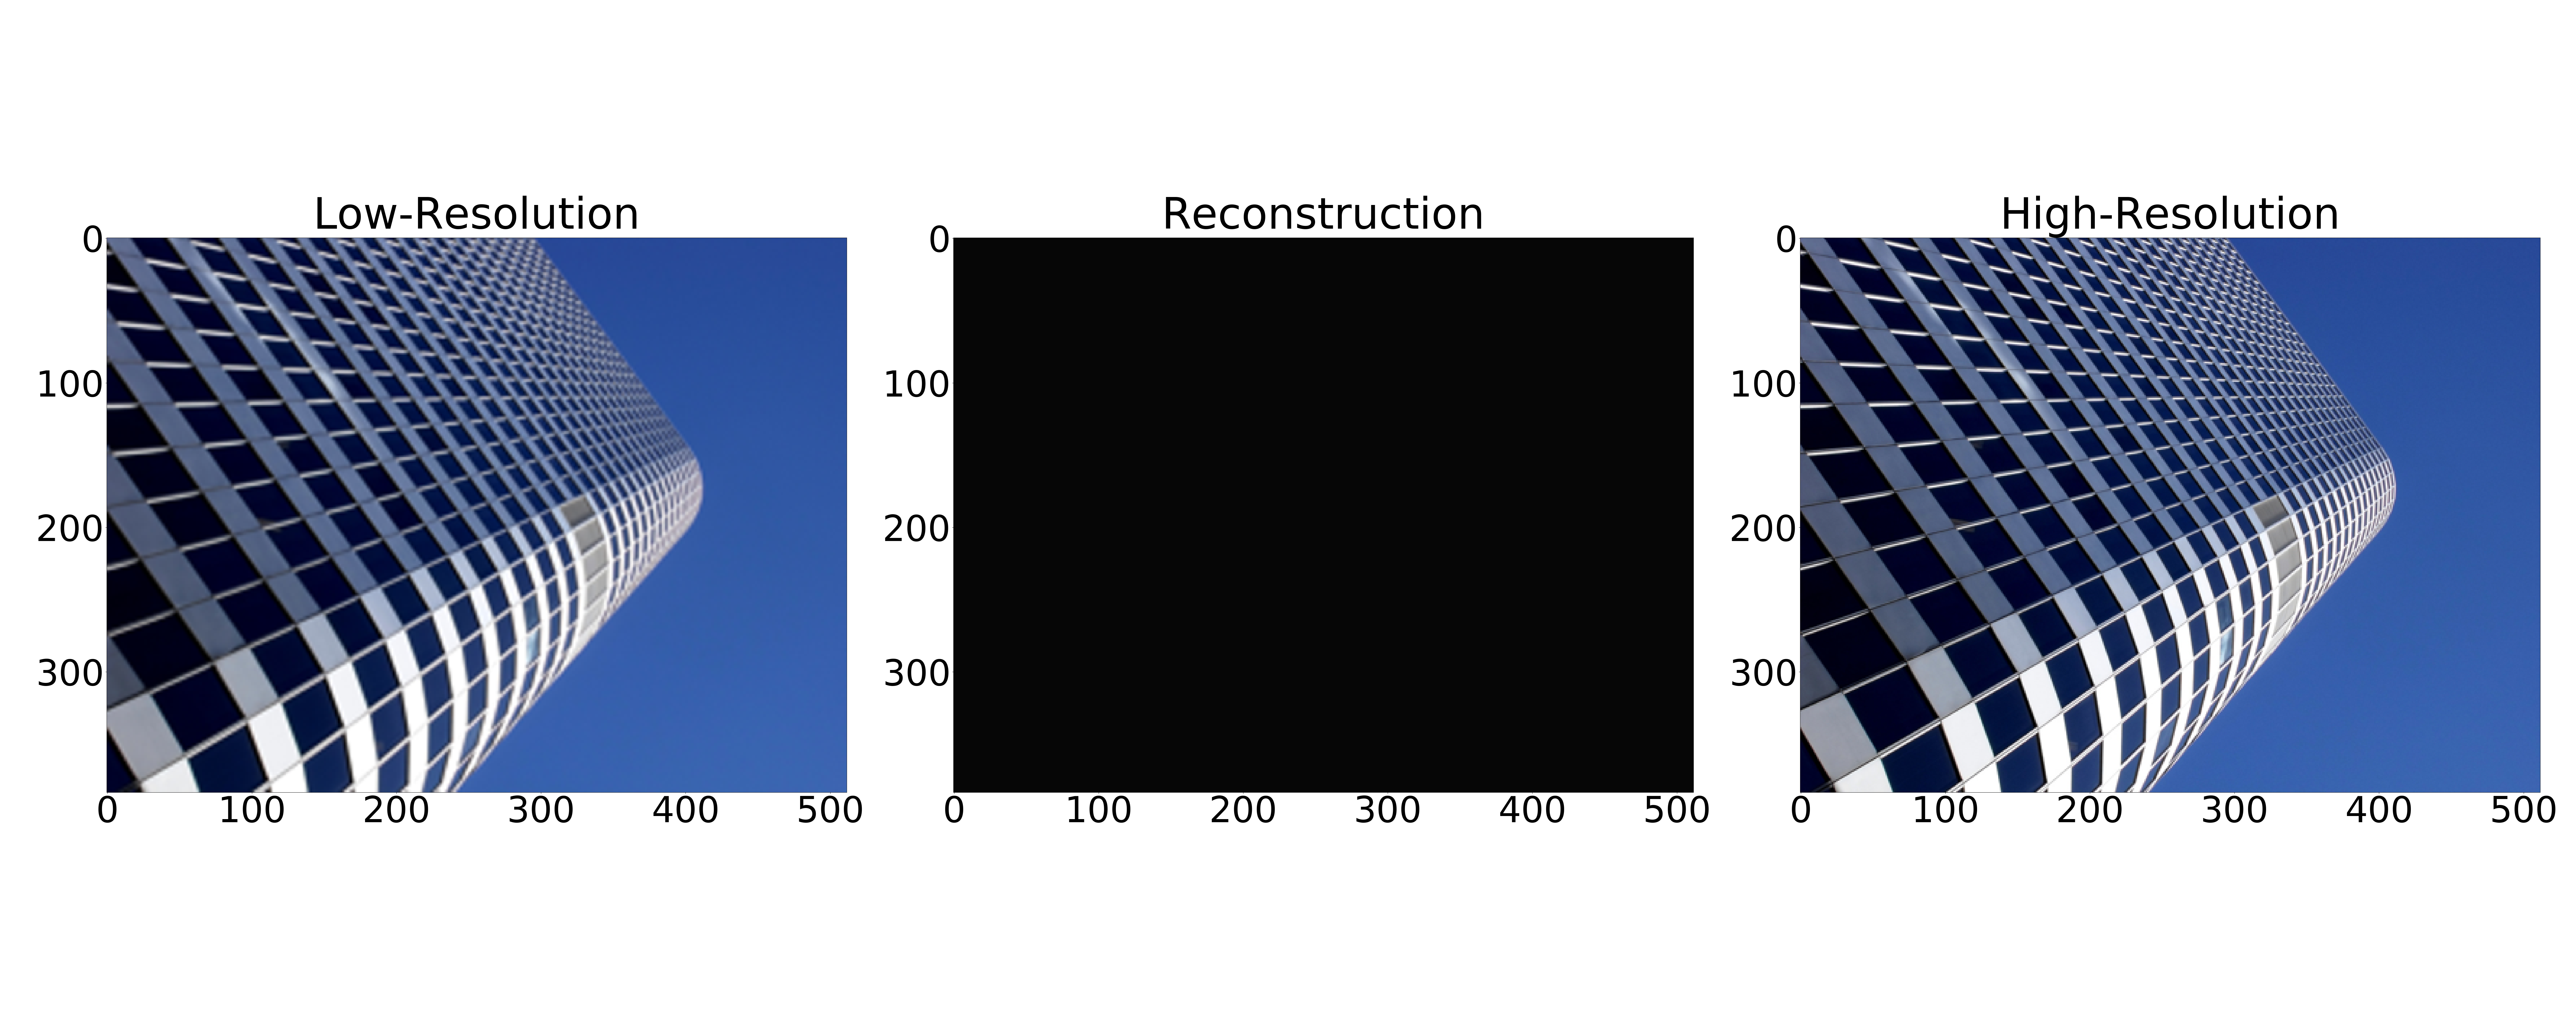
\includegraphics{4_psnr_7.png}
\caption{Reconstruction after 4 epochs\label{epochs_low}}
\end{figure}

\begin{figure}
\centering
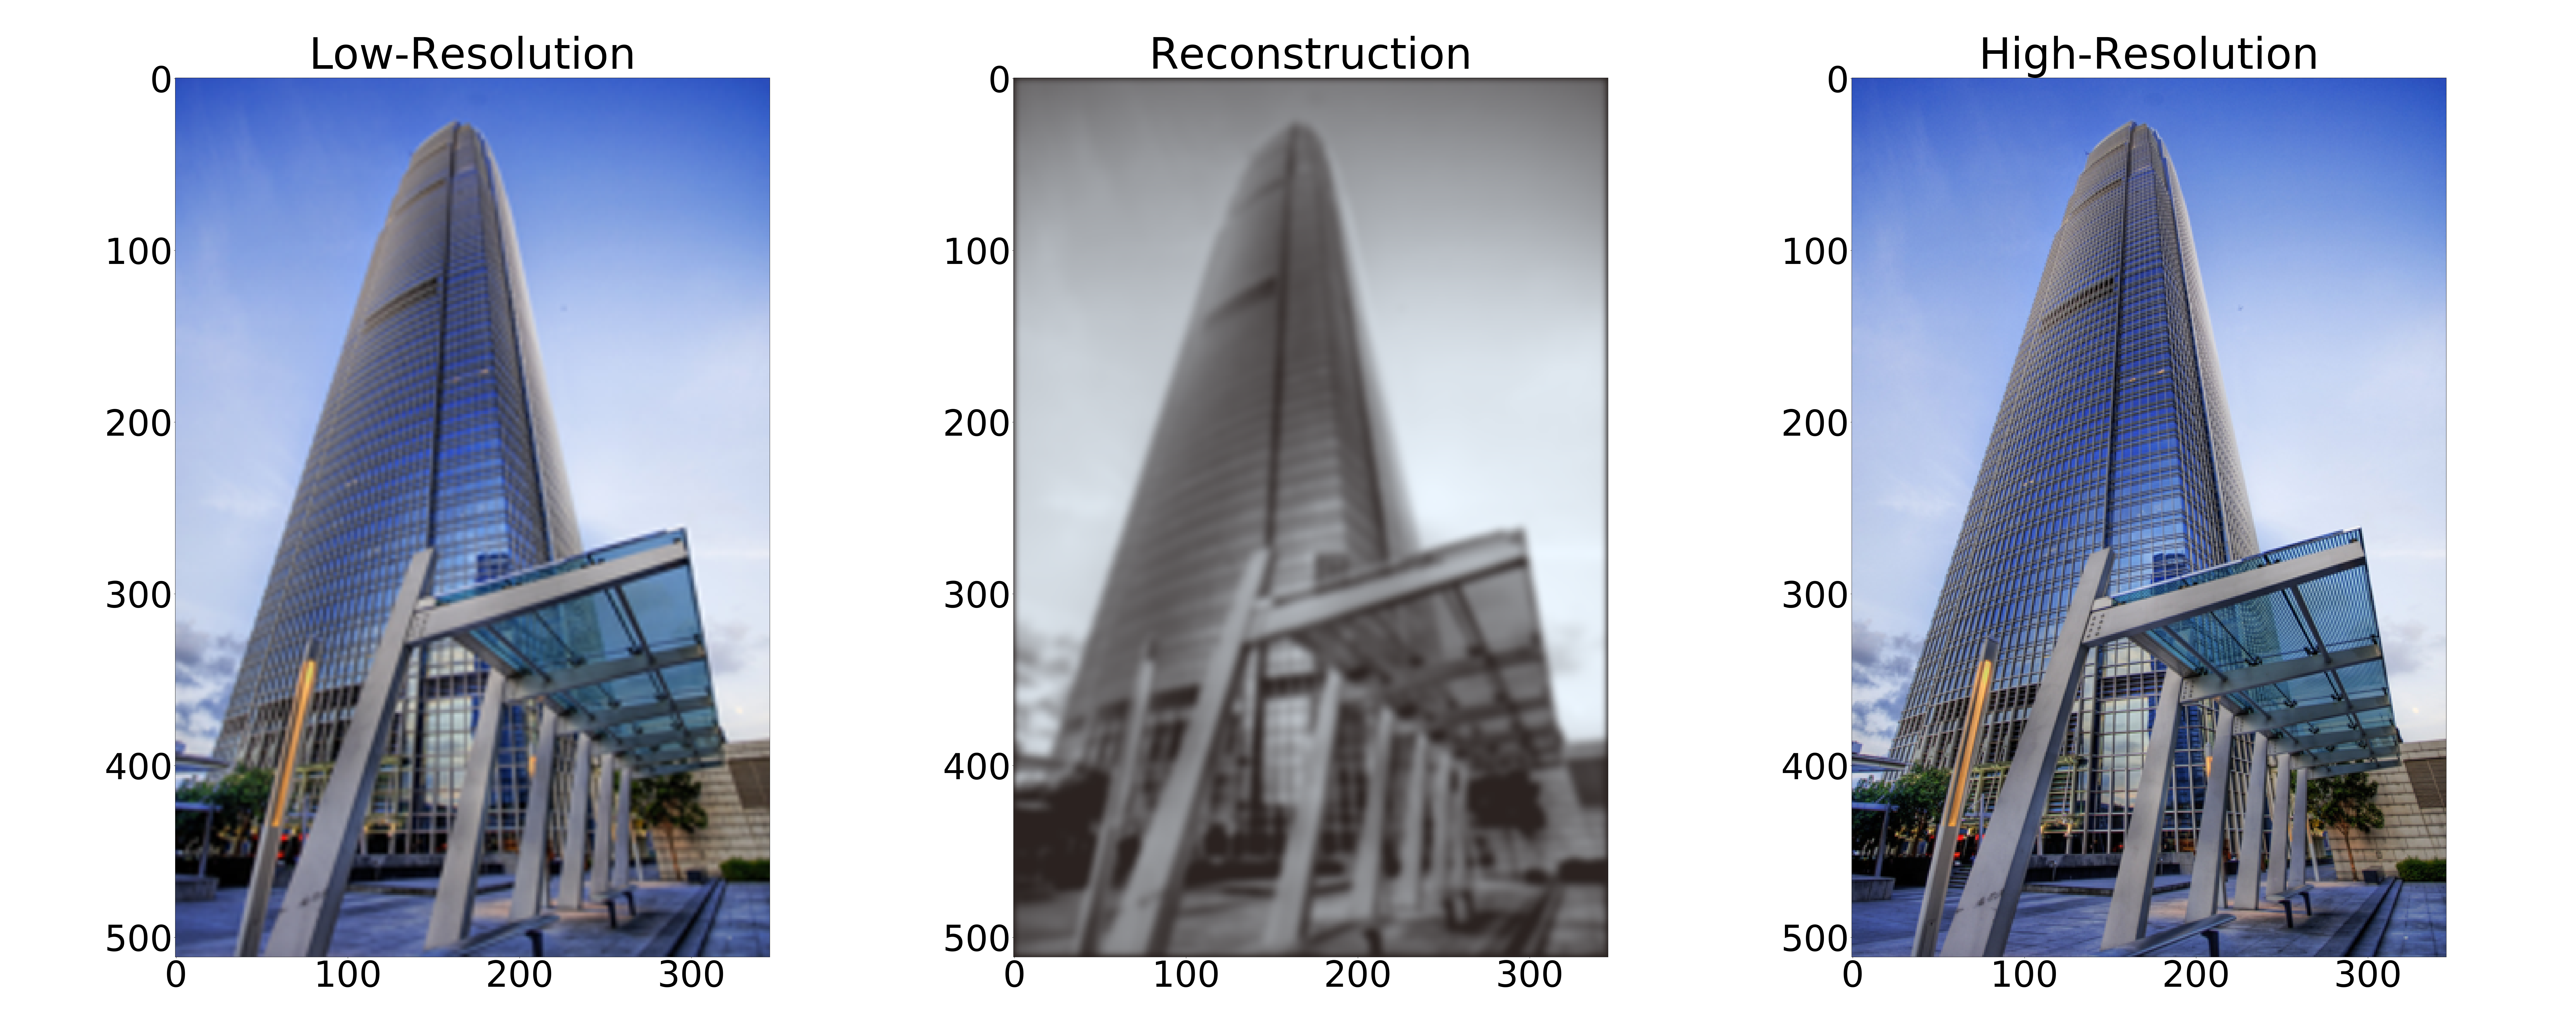
\includegraphics{531_psnr_17.png}
\caption{Reconstruction after 531 epochs\label{epochs_medium}}
\end{figure}

\begin{figure}
\centering
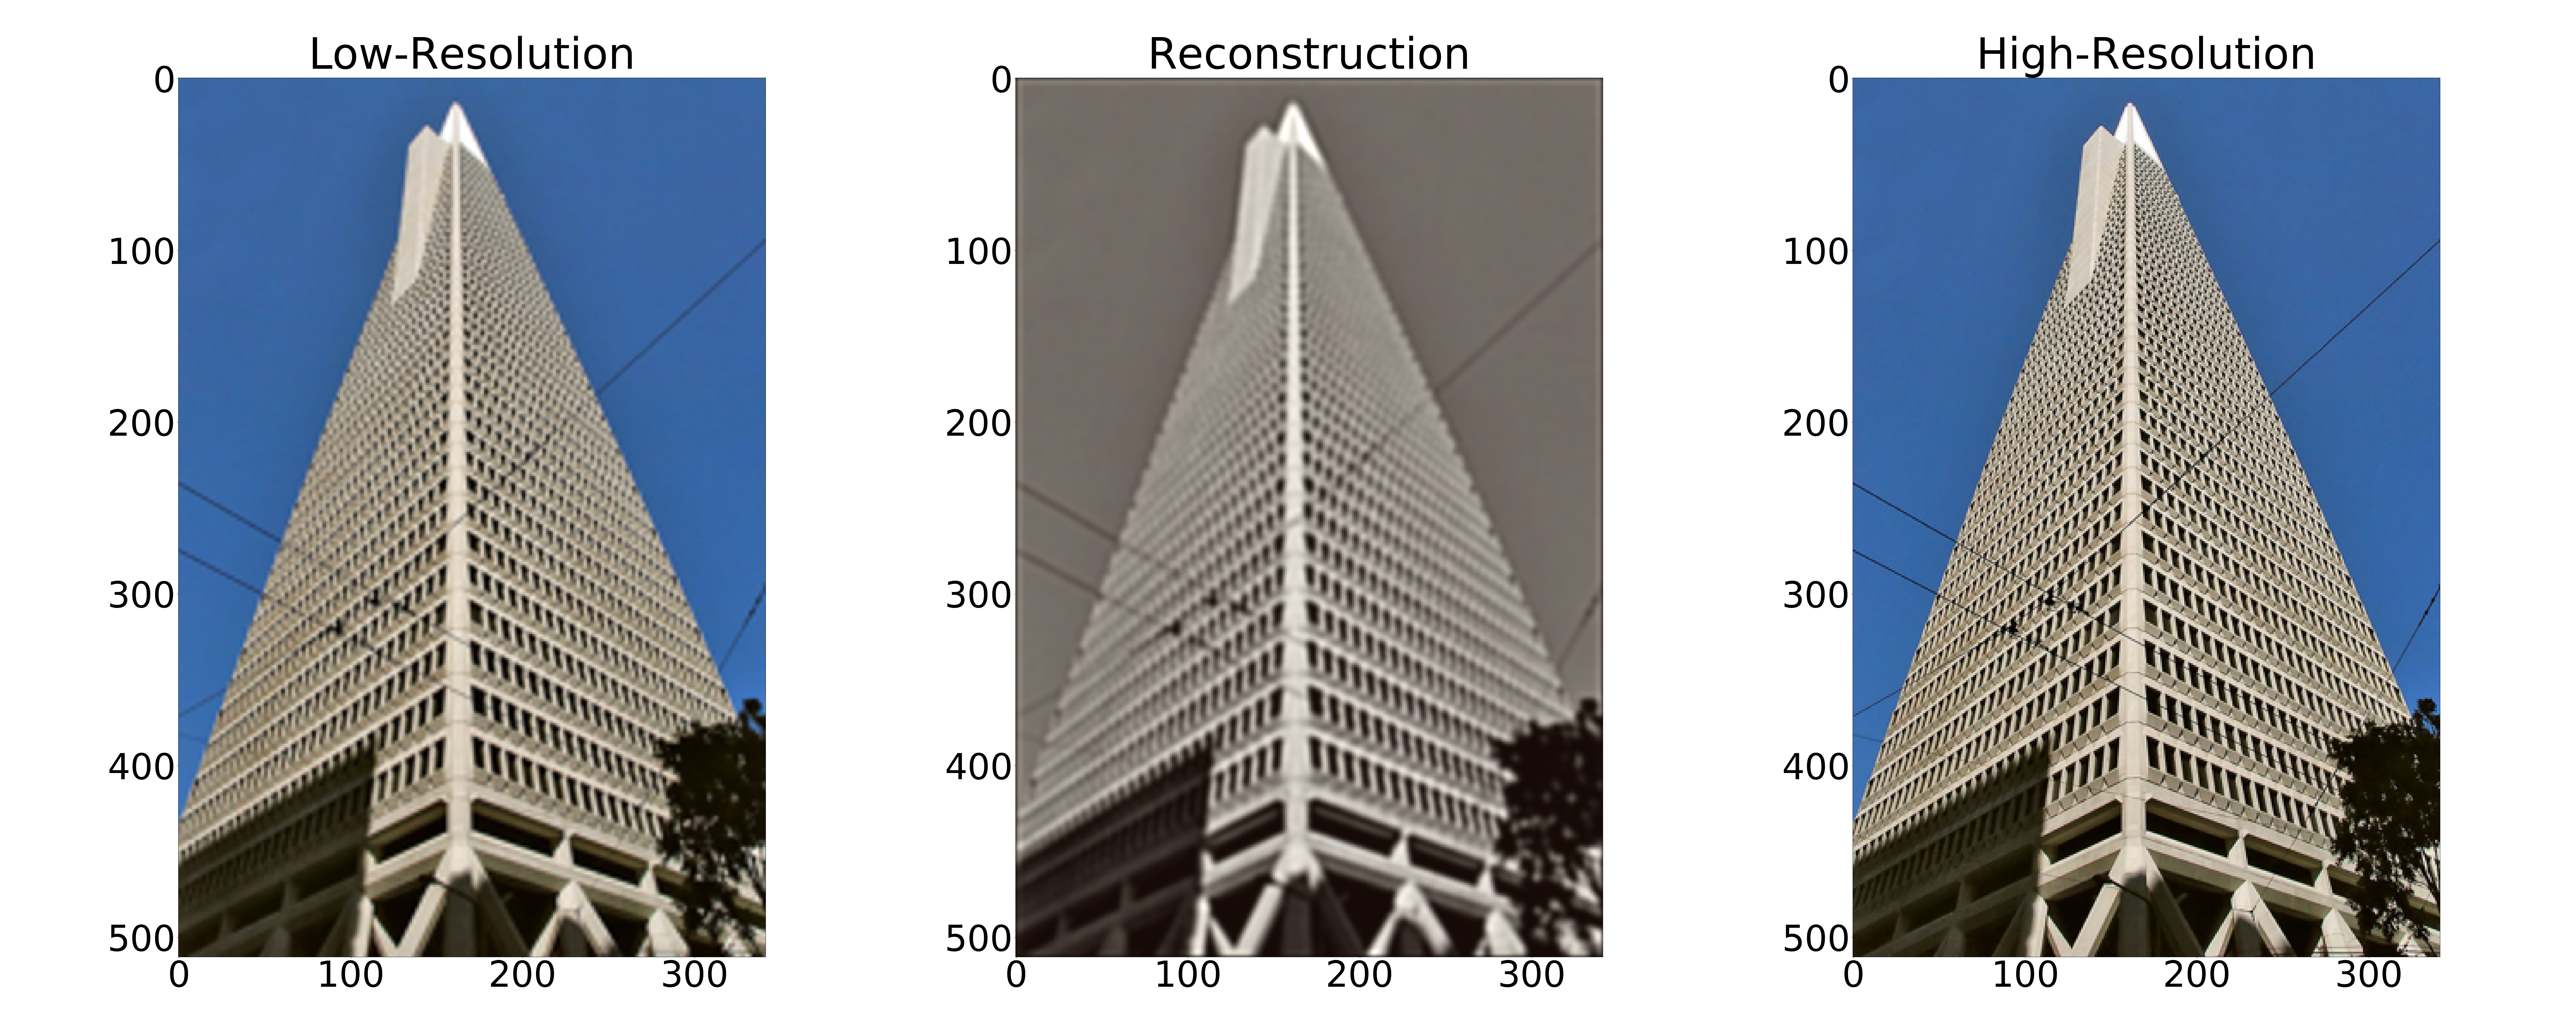
\includegraphics{1184_psnr_15.png}
\caption{Reconstruction after 1184 epochs\label{epochs_high}}
\end{figure}

\hypertarget{deliver}{%
\subsection{Deliver}\label{deliver}}

Finally, after some research I found another SR network based on (Ledig
et al. 2016) with a Github
repository\footnote{\url{https://github.com/krasserm/super-resolution}, seen on 2020-01-22}
which is implemented in Tensorflow
2\footnote{\url{https://www.tensorflow.org/}, seen on 2020-01-22}. The
codebase provides some Jupyter notebooks to train and test the weights
and also contains links to weights for immediate usage.

On top of this I implemented a simple, client/server web application
(based on
FLASK\footnote{\url{https://www.palletsprojects.com/p/flask/}, seen on 2020-01-22}
see screenshot \ref{screenshot}) which allows the upload of a low
resolution PNG image which gets upscaled by using a SR-GAN and a simple
bilinear upscaling as benchmark. Both images are displayed next to
another for comparion.

The web application sends the low resolution image to the backend which
does the upscaling. The decision to upscale on the backend was driven by
the fact, that the model can easier be used in the same environment as
it was trained: Python + Tensorflow 2. For the frontend implementation,
simple HTML and JS were used.

Nevertheless the application looses its desired advantage to handle
everything in the frontend.

\begin{figure}
\centering
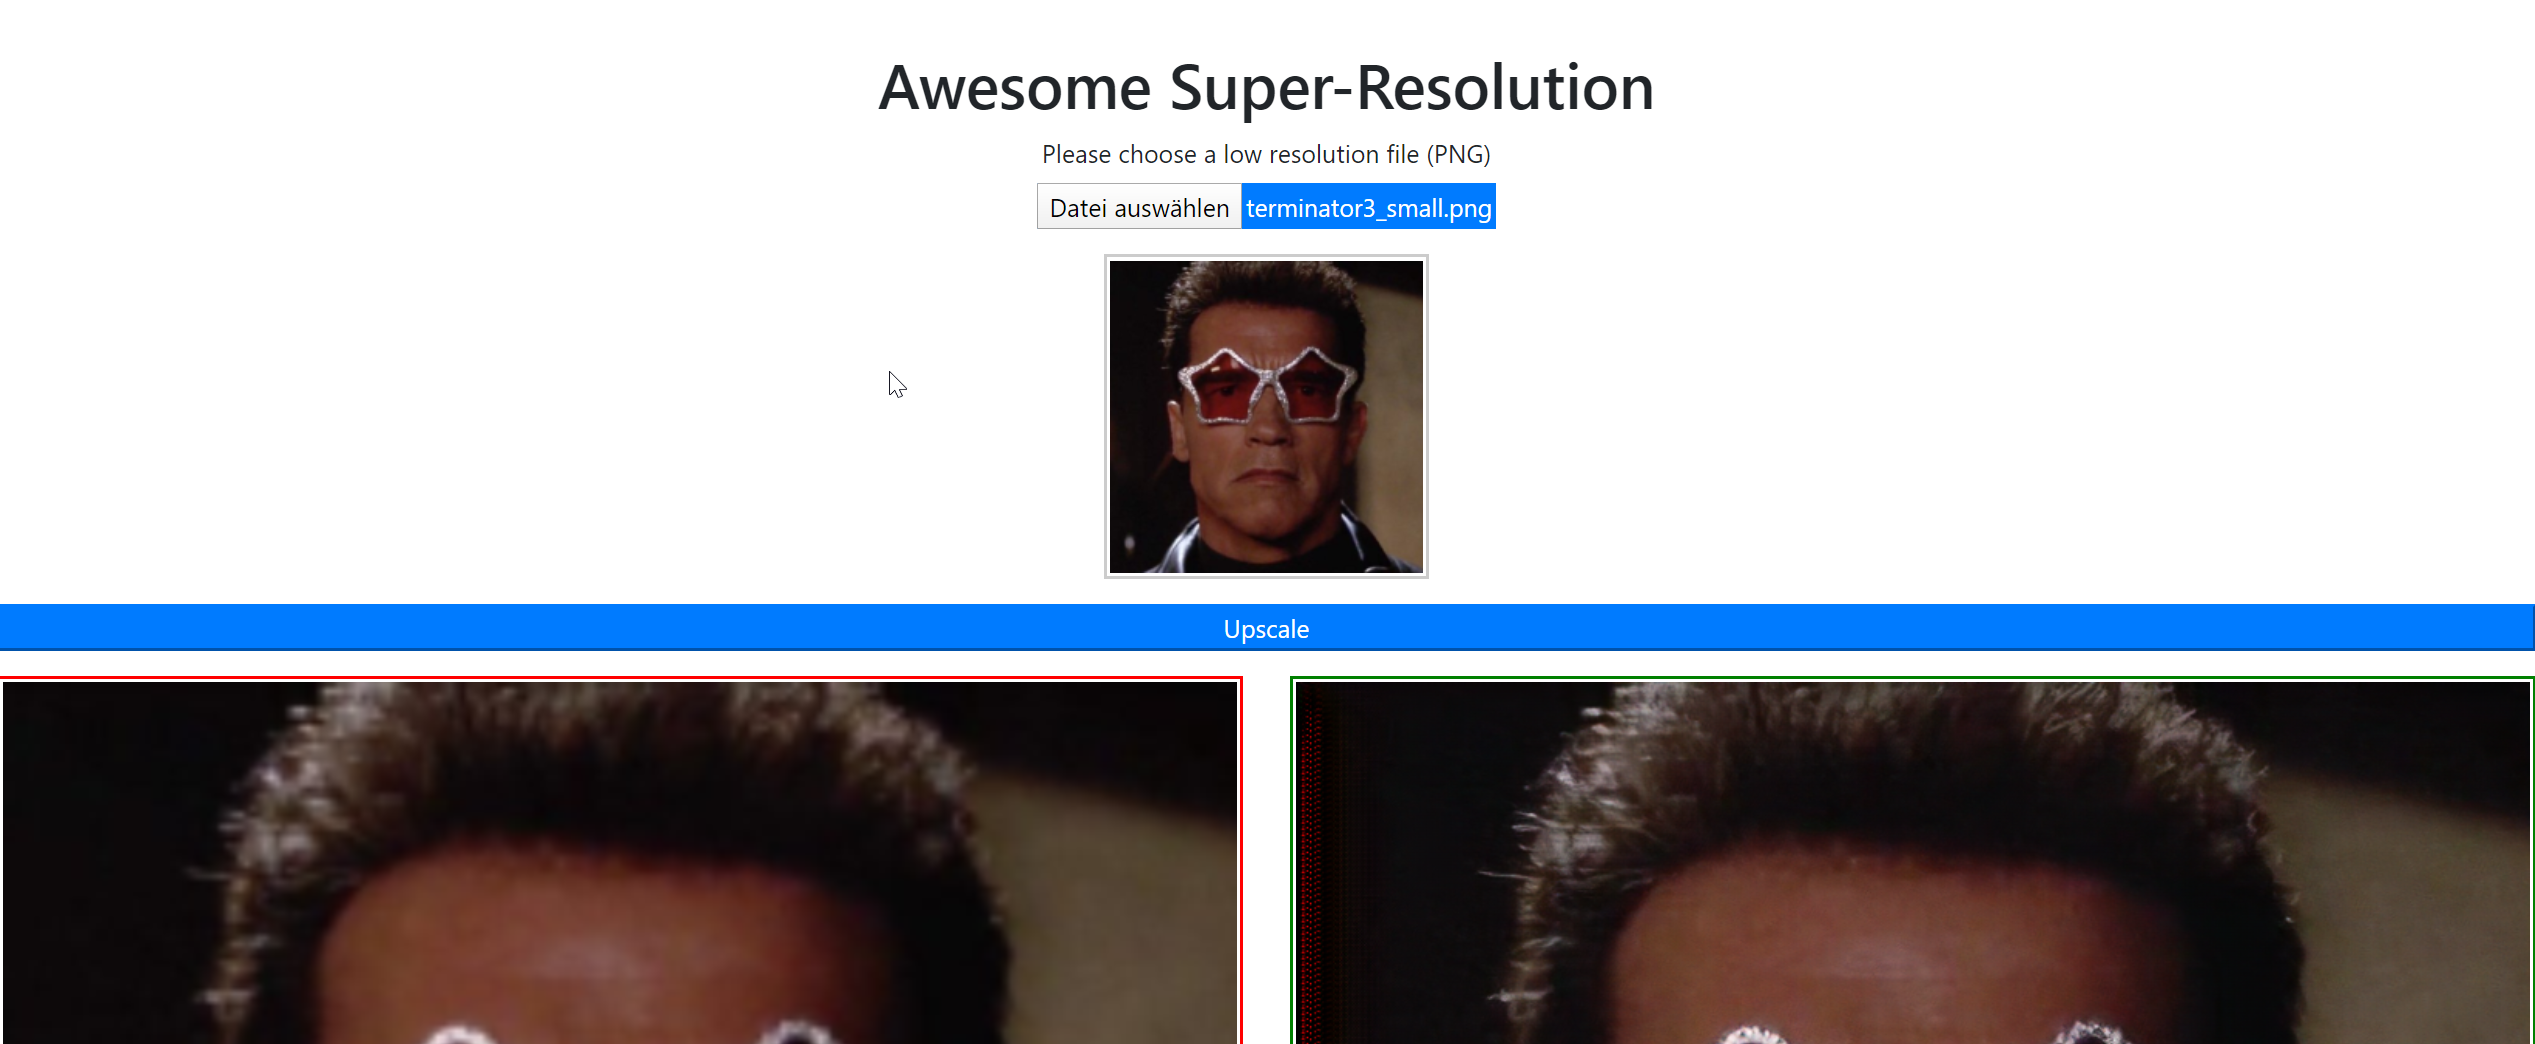
\includegraphics{screenshot.png}
\caption{Screenshot of the web application\label{screenshot}}
\end{figure}

The source code an a more detailed description is available on
Github\footnote{\url{https://github.com/websta/AppliedDeeplearning}, seen on 2020-01-22}
and contains a dockerfile to pack everything together which is required
to run the Super-Awesome Super-Resolution.

\hypertarget{take-aways}{%
\subsection{Take-aways}\label{take-aways}}

My main take-aways are:

\begin{itemize}
\item
  Neural networks are not that scary, as it seems, I am still wondering
  how someone can come up with the network structure. Probaly I need to
  see more networks to get an idea.
\item
  Setting up GPU based learning is not that easy, even you have a
  tutorial.
\item
  Using the network needs information about the format of the required
  input. Could not find that for existing models on
  ModelZoo\footnote{\url{https://modelzoo.co/}, seen on 2020-01-22}.
\item
  Probably the simples use of a neural network is to put it into the
  same environment as it was trained (Python and Tensorflow 2 in my
  case) and attach some REST endoints.
\end{itemize}

\hypertarget{effort}{%
\section{Effort}\label{effort}}

For the 3 phases of the project, these are my time spent (roughly):

\begin{itemize}
\tightlist
\item
  Initiate: 3 hours research, report
\item
  Hacking: 40 hours translating code to Colab, Google Drive integration,
  rerun training on Colab, provisioning and installing Cuda on Azure VM,
  training on CPU, collecting and interpret results, tries to convert
  model to tensorflow.js, tries to use another model, report
\item
  Delivery: 20 hours creating a web application (client/server), testing
  \& minimal style, dockerfile, report
\end{itemize}

\hypertarget{references}{%
\section*{References}\label{references}}
\addcontentsline{toc}{section}{References}

\hypertarget{refs}{}
\leavevmode\hypertarget{ref-DBLP:journalsux2fcorrux2fLedigTHCATTWS16}{}%
Ledig, Christian, Lucas Theis, Ferenc Huszar, Jose Caballero, Andrew P.
Aitken, Alykhan Tejani, Johannes Totz, Zehan Wang, and Wenzhe Shi. 2016.
``Photo-Realistic Single Image Super-Resolution Using a Generative
Adversarial Network.'' \emph{CoRR} abs/1609.04802.
\url{http://arxiv.org/abs/1609.04802}.

\leavevmode\hypertarget{ref-DBLP:journalsux2fcorrux2fabs-1804-02900}{}%
Wang, Yifan, Federico Perazzi, Brian McWilliams, Alexander
Sorkine-Hornung, Olga Sorkine-Hornung, and Christopher Schroers. 2018.
``A Fully Progressive Approach to Single-Image Super-Resolution.''
\emph{CoRR} abs/1804.02900. \url{http://arxiv.org/abs/1804.02900}.


\end{document}
